
%% bare_conf_compsoc.tex
%% V1.4a
%% 2014/09/17
%% by Michael Shell
%% See:
%% http://www.michaelshell.org/
%% for current contact information.
%%
%% This is a skeleton file demonstrating the use of IEEEtran.cls
%% (requires IEEEtran.cls version 1.8s or later) with an IEEE Computer
%% Society conference paper.
%%
%% Support sites:
%% http://www.michaelshell.org/tex/ieeetran/
%% http://www.ctan.org/tex-archive/macros/latex/contrib/IEEEtran/
%% and
%% http://www.ieee.org/

%%*************************************************************************
%% Legal Notice:
%% This code is offered as-is without any warranty either expressed or
%% implied; without even the implied warranty of MERCHANTABILITY or
%% FITNESS FOR A PARTICULAR PURPOSE! 
%% User assumes all risk.
%% In no event shall IEEE or any contributor to this code be liable for
%% any damages or losses, including, but not limited to, incidental,
%% consequential, or any other damages, resulting from the use or misuse
%% of any information contained here.
%%
%% All comments are the opinions of their respective authors and are not
%% necessarily endorsed by the IEEE.
%%
%% This work is distributed under the LaTeX Project Public License (LPPL)
%% ( http://www.latex-project.org/ ) version 1.3, and may be freely used,
%% distributed and modified. A copy of the LPPL, version 1.3, is included
%% in the base LaTeX documentation of all distributions of LaTeX released
%% 2003/12/01 or later.
%% Retain all contribution notices and credits.
%% ** Modified files should be clearly indicated as such, including  **
%% ** renaming them and changing author support contact information. **
%%
%% File list of work: IEEEtran.cls, IEEEtran_HOWTO.pdf, bare_adv.tex,
%%                    bare_conf.tex, bare_jrnl.tex, bare_conf_compsoc.tex,
%%                    bare_jrnl_compsoc.tex, bare_jrnl_transmag.tex
%%*************************************************************************


% *** Authors should verify (and, if needed, correct) their LaTeX system  ***
% *** with the testflow diagnostic prior to trusting their LaTeX platform ***
% *** with production work. IEEE's font choices and paper sizes can       ***
% *** trigger bugs that do not appear when using other class files.       ***                          ***
% The testflow support page is at:
% http://www.michaelshell.org/tex/testflow/



\documentclass[conference,compsoc]{IEEEtran}
% Some/most Computer Society conferences require the compsoc mode option,
% but others may want the standard conference format.
%
% If IEEEtran.cls has not been installed into the LaTeX system files,
% manually specify the path to it like:
% \documentclass[conference,compsoc]{../sty/IEEEtran}

\usepackage{algorithm}
\usepackage{algpseudocode}
\usepackage{amsmath}
\usepackage{graphicx}
\usepackage{url}
\newcommand{\pluseq}{\mathrel{+}=}
\newcommand{\asteq}{\mathrel{*}=}



% Some very useful LaTeX packages include:
% (uncomment the ones you want to load)


% *** MISC UTILITY PACKAGES ***
%
%\usepackage{ifpdf}
% Heiko Oberdiek's ifpdf.sty is very useful if you need conditional
% compilation based on whether the output is pdf or dvi.
% usage:
% \ifpdf
%   % pdf code
% \else
%   % dvi code
% \fi
% The latest version of ifpdf.sty can be obtained from:
% http://www.ctan.org/tex-archive/macros/latex/contrib/oberdiek/
% Also, note that IEEEtran.cls V1.7 and later provides a builtin
% \ifCLASSINFOpdf conditional that works the same way.
% When switching from latex to pdflatex and vice-versa, the compiler may
% have to be run twice to clear warning/error messages.






% *** CITATION PACKAGES ***
%
\ifCLASSOPTIONcompsoc
  % IEEE Computer Society needs nocompress option
  % requires cite.sty v4.0 or later (November 2003)
  \usepackage[nocompress]{cite}
\else
  % normal IEEE
  \usepackage{cite}
\fi
% cite.sty was written by Donald Arseneau
% V1.6 and later of IEEEtran pre-defines the format of the cite.sty package
% \cite{} output to follow that of IEEE. Loading the cite package will
% result in citation numbers being automatically sorted and properly
% "compressed/ranged". e.g., [1], [9], [2], [7], [5], [6] without using
% cite.sty will become [1], [2], [5]--[7], [9] using cite.sty. cite.sty's
% \cite will automatically add leading space, if needed. Use cite.sty's
% noadjust option (cite.sty V3.8 and later) if you want to turn this off
% such as if a citation ever needs to be enclosed in parenthesis.
% cite.sty is already installed on most LaTeX systems. Be sure and use
% version 5.0 (2009-03-20) and later if using hyperref.sty.
% The latest version can be obtained at:
% http://www.ctan.org/tex-archive/macros/latex/contrib/cite/
% The documentation is contained in the cite.sty file itself.
%
% Note that some packages require special options to format as the Computer
% Society requires. In particular, Computer Society  papers do not use
% compressed citation ranges as is done in typical IEEE papers
% (e.g., [1]-[4]). Instead, they list every citation separately in order
% (e.g., [1], [2], [3], [4]). To get the latter we need to load the cite
% package with the nocompress option which is supported by cite.sty v4.0
% and later.





% *** GRAPHICS RELATED PACKAGES ***
%
\ifCLASSINFOpdf
  % \usepackage[pdftex]{graphicx}
  % declare the path(s) where your graphic files are
  % \graphicspath{{../pdf/}{../jpeg/}}
  % and their extensions so you won't have to specify these with
  % every instance of \includegraphics
  % \DeclareGraphicsExtensions{.pdf,.jpeg,.png}
\else
  % or other class option (dvipsone, dvipdf, if not using dvips). graphicx
  % will default to the driver specified in the system graphics.cfg if no
  % driver is specified.
  % \usepackage[dvips]{graphicx}
  % declare the path(s) where your graphic files are
  % \graphicspath{{../eps/}}
  % and their extensions so you won't have to specify these with
  % every instance of \includegraphics
  % \DeclareGraphicsExtensions{.eps}
\fi
% graphicx was written by David Carlisle and Sebastian Rahtz. It is
% required if you want graphics, photos, etc. graphicx.sty is already
% installed on most LaTeX systems. The latest version and documentation
% can be obtained at: 
% http://www.ctan.org/tex-archive/macros/latex/required/graphics/
% Another good source of documentation is "Using Imported Graphics in
% LaTeX2e" by Keith Reckdahl which can be found at:
% http://www.ctan.org/tex-archive/info/epslatex/
%
% latex, and pdflatex in dvi mode, support graphics in encapsulated
% postscript (.eps) format. pdflatex in pdf mode supports graphics
% in .pdf, .jpeg, .png and .mps (metapost) formats. Users should ensure
% that all non-photo figures use a vector format (.eps, .pdf, .mps) and
% not a bitmapped formats (.jpeg, .png). IEEE frowns on bitmapped formats
% which can result in "jaggedy"/blurry rendering of lines and letters as
% well as large increases in file sizes.
%
% You can find documentation about the pdfTeX application at:
% http://www.tug.org/applications/pdftex





% *** MATH PACKAGES ***
%
%\usepackage[cmex10]{amsmath}
% A popular package from the American Mathematical Society that provides
% many useful and powerful commands for dealing with mathematics. If using
% it, be sure to load this package with the cmex10 option to ensure that
% only type 1 fonts will utilized at all point sizes. Without this option,
% it is possible that some math symbols, particularly those within
% footnotes, will be rendered in bitmap form which will result in a
% document that can not be IEEE Xplore compliant!
%
% Also, note that the amsmath package sets \interdisplaylinepenalty to 10000
% thus preventing page breaks from occurring within multiline equations. Use:
%\interdisplaylinepenalty=2500
% after loading amsmath to restore such page breaks as IEEEtran.cls normally
% does. amsmath.sty is already installed on most LaTeX systems. The latest
% version and documentation can be obtained at:
% http://www.ctan.org/tex-archive/macros/latex/required/amslatex/math/





% *** SPECIALIZED LIST PACKAGES ***
%
%\usepackage{algorithmic}
% algorithmic.sty was written by Peter Williams and Rogerio Brito.
% This package provides an algorithmic environment fo describing algorithms.
% You can use the algorithmic environment in-text or within a figure
% environment to provide for a floating algorithm. Do NOT use the algorithm
% floating environment provided by algorithm.sty (by the same authors) or
% algorithm2e.sty (by Christophe Fiorio) as IEEE does not use dedicated
% algorithm float types and packages that provide these will not provide
% correct IEEE style captions. The latest version and documentation of
% algorithmic.sty can be obtained at:
% http://www.ctan.org/tex-archive/macros/latex/contrib/algorithms/
% There is also a support site at:
% http://algorithms.berlios.de/index.html
% Also of interest may be the (relatively newer and more customizable)
% algorithmicx.sty package by Szasz Janos:
% http://www.ctan.org/tex-archive/macros/latex/contrib/algorithmicx/




% *** ALIGNMENT PACKAGES ***
%
%\usepackage{array}
% Frank Mittelbach's and David Carlisle's array.sty patches and improves
% the standard LaTeX2e array and tabular environments to provide better
% appearance and additional user controls. As the default LaTeX2e table
% generation code is lacking to the point of almost being broken with
% respect to the quality of the end results, all users are strongly
% advised to use an enhanced (at the very least that provided by array.sty)
% set of table tools. array.sty is already installed on most systems. The
% latest version and documentation can be obtained at:
% http://www.ctan.org/tex-archive/macros/latex/required/tools/


% IEEEtran contains the IEEEeqnarray family of commands that can be used to
% generate multiline equations as well as matrices, tables, etc., of high
% quality.




% *** SUBFIGURE PACKAGES ***
%\ifCLASSOPTIONcompsoc
%  \usepackage[caption=false,font=footnotesize,labelfont=sf,textfont=sf]{subfig}
%\else
%  \usepackage[caption=false,font=footnotesize]{subfig}
%\fi
% subfig.sty, written by Steven Douglas Cochran, is the modern replacement
% for subfigure.sty, the latter of which is no longer maintained and is
% incompatible with some LaTeX packages including fixltx2e. However,
% subfig.sty requires and automatically loads Axel Sommerfeldt's caption.sty
% which will override IEEEtran.cls' handling of captions and this will result
% in non-IEEE style figure/table captions. To prevent this problem, be sure
% and invoke subfig.sty's "caption=false" package option (available since
% subfig.sty version 1.3, 2005/06/28) as this is will preserve IEEEtran.cls
% handling of captions.
% Note that the Computer Society format requires a sans serif font rather
% than the serif font used in traditional IEEE formatting and thus the need
% to invoke different subfig.sty package options depending on whether
% compsoc mode has been enabled.
%
% The latest version and documentation of subfig.sty can be obtained at:
% http://www.ctan.org/tex-archive/macros/latex/contrib/subfig/




% *** FLOAT PACKAGES ***
%
%\usepackage{fixltx2e}
% fixltx2e, the successor to the earlier fix2col.sty, was written by
% Frank Mittelbach and David Carlisle. This package corrects a few problems
% in the LaTeX2e kernel, the most notable of which is that in current
% LaTeX2e releases, the ordering of single and double column floats is not
% guaranteed to be preserved. Thus, an unpatched LaTeX2e can allow a
% single column figure to be placed prior to an earlier double column
% figure. The latest version and documentation can be found at:
% http://www.ctan.org/tex-archive/macros/latex/base/


%\usepackage{stfloats}
% stfloats.sty was written by Sigitas Tolusis. This package gives LaTeX2e
% the ability to do double column floats at the bottom of the page as well
% as the top. (e.g., "\begin{figure*}[!b]" is not normally possible in
% LaTeX2e). It also provides a command:
%\fnbelowfloat
% to enable the placement of footnotes below bottom floats (the standard
% LaTeX2e kernel puts them above bottom floats). This is an invasive package
% which rewrites many portions of the LaTeX2e float routines. It may not work
% with other packages that modify the LaTeX2e float routines. The latest
% version and documentation can be obtained at:
% http://www.ctan.org/tex-archive/macros/latex/contrib/sttools/
% Do not use the stfloats baselinefloat ability as IEEE does not allow
% \baselineskip to stretch. Authors submitting work to the IEEE should note
% that IEEE rarely uses double column equations and that authors should try
% to avoid such use. Do not be tempted to use the cuted.sty or midfloat.sty
% packages (also by Sigitas Tolusis) as IEEE does not format its papers in
% such ways.
% Do not attempt to use stfloats with fixltx2e as they are incompatible.
% Instead, use Morten Hogholm'a dblfloatfix which combines the features
% of both fixltx2e and stfloats:
%
% \usepackage{dblfloatfix}
% The latest version can be found at:
% http://www.ctan.org/tex-archive/macros/latex/contrib/dblfloatfix/




% *** PDF, URL AND HYPERLINK PACKAGES ***
%
%\usepackage{url}
% url.sty was written by Donald Arseneau. It provides better support for
% handling and breaking URLs. url.sty is already installed on most LaTeX
% systems. The latest version and documentation can be obtained at:
% http://www.ctan.org/tex-archive/macros/latex/contrib/url/
% Basically, \url{my_url_here}.




% *** Do not adjust lengths that control margins, column widths, etc. ***
% *** Do not use packages that alter fonts (such as pslatex).         ***
% There should be no need to do such things with IEEEtran.cls V1.6 and later.
% (Unless specifically asked to do so by the journal or conference you plan
% to submit to, of course. )


% correct bad hyphenation here
\hyphenation{op-tical net-works semi-conduc-tor}


\begin{document}
%
% paper title
% Titles are generally capitalized except for words such as a, an, and, as,
% at, but, by, for, in, nor, of, on, or, the, to and up, which are usually
% not capitalized unless they are the first or last word of the title.
% Linebreaks \\ can be used within to get better formatting as desired.
% Do not put math or special symbols in the title.
\title{Topic-Aware Sentiment Prediction for Chinese ConceptNet}


% author names and affiliations
% use a multiple column layout for up to three different
% affiliations
\author{
\IEEEauthorblockN{Po-Hao Chou\IEEEauthorrefmark{1},
Chi-Chia Huang\IEEEauthorrefmark{2}, Richard Tzong-Han Tsai\IEEEauthorrefmark{3} and
Jane Yung-jen Hsu\IEEEauthorrefmark{4}}

\IEEEauthorblockA{
\IEEEauthorrefmark{1}\IEEEauthorrefmark{2}\IEEEauthorrefmark{4}Computer Science and Information Engineering, National Taiwan University \\
\IEEEauthorrefmark{3}Computer Science and Information Engineering, National Central University \\
Email: \{
\IEEEauthorrefmark{1}r02922017, \IEEEauthorrefmark{2}d01944003,
\IEEEauthorrefmark{4}yjhsu\}@csie.ntu.edu.tw
\IEEEauthorrefmark{3}thtsai@csie.ncu.edu.tw}
}

% conference papers do not typically use \thanks and this command
% is locked out in conference mode. If really needed, such as for
% the acknowledgment of grants, issue a \IEEEoverridecommandlockouts
% after \documentclass

% for over three affiliations, or if they all won't fit within the width
% of the page (and note that there is less available width in this regard for
% compsoc conferences compared to traditional conferences), use this
% alternative format:
% 
%\author{\IEEEauthorblockN{Michael Shell\IEEEauthorrefmark{1},
%Homer Simpson\IEEEauthorrefmark{2},
%James Kirk\IEEEauthorrefmark{3}, 
%Montgomery Scott\IEEEauthorrefmark{3} and
%Eldon Tyrell\IEEEauthorrefmark{4}}
%\IEEEauthorblockA{\IEEEauthorrefmark{1}School of Electrical and Computer Engineering\\
%Georgia Institute of Technology,
%Atlanta, Georgia 30332--0250\\ Email: see http://www.michaelshell.org/contact.html}
%\IEEEauthorblockA{\IEEEauthorrefmark{2}Twentieth Century Fox, Springfield, USA\\
%Email: homer@thesimpsons.com}
%\IEEEauthorblockA{\IEEEauthorrefmark{3}Starfleet Academy, San Francisco, California 96678-2391\\
%Telephone: (800) 555--1212, Fax: (888) 555--1212}
%\IEEEauthorblockA{\IEEEauthorrefmark{4}Tyrell Inc., 123 Replicant Street, Los Angeles, California 90210--4321}}




% use for special paper notices
%\IEEEspecialpapernotice{(Invited Paper)}




% make the title area
\maketitle

% As a general rule, do not put math, special symbols or citations
% in the abstract
\begin{abstract}
Sentiment dictionary is a valuable resource in sentiment analysis research. Previous work propagate sentiment values from existing high quality dictionary on semantic networks to build wide coverage dictionary efficiently. But this approach suffers from quality degradation during propagation. In this work, we propose a topic-aware propagation method on Chinese ConceptNet to ease the issue. The experiment result shows that the generated topic-aware sentiment dictionary help improve the performance of polarity classification for texts.


% It is difficult obtain wide coverage dictionary with high quality sentiment values.

%Sentiment analysis aims to identify the attitudes or emotions behind texts. For many sentiment analysis approaches, sentiment information of terms or phrases plays an important role. However, in Chinese sentiment analysis, the coverage of such information is still limited. To increase the coverage, some methods has been developed to predict sentiments for nodes in Chinese ConceptNet due to its large size and high semantic level nodes. In ConceptNet, the notion of a node is extended from purely lexical terms to include higher-order compound concepts, e.g., `eat lunch', `satisfy hunger', so these nodes are called concepts. 

%Current approaches aim to assign one sentiment to each concept, but in fact a concept may have different sentiments on different contexts, such as `scream' and `sudden' in Chinese. In this paper, our first goal is to extract the hidden contextual information in Chinese ConceptNet and use it to estimate sentiments in different situations for each concept. To achieve this goal, we propose a topic-aware sentiment propagation approach. We apply Latent Dirichlet Allocation to divide Chinese ConceptNet into different topic layers and use sentiment propagation on each topic layer to predict topic-aware sentiments for Chinese concepts. Our another goal is to use the generated topic-aware sentiments of concepts to improve the polarity classification for texts. We combine other co-occurring concepts to identify topics and select sentiments for concepts in texts. Then, experiments conducted on dialogue dataset and microblog posts show the improvement of topic-aware prediction for concepts and texts. 
\end{abstract}

% no keywords




% For peer review papers, you can put extra information on the cover
% page as needed:
% \ifCLASSOPTIONpeerreview
% \begin{center} \bfseries EDICS Category: 3-BBND \end{center}
% \fi
%
% For peerreview papers, this IEEEtran command inserts a page break and
% creates the second title. It will be ignored for other modes.
\IEEEpeerreviewmaketitle



\section{Introduction}
\label{sec:introduction}
With the rise of social media services, more and more people share their opinions, feelings, experiences on the web. The roles of users shift from information consumers to information producers. To understand the attitudes and emotions behind these texts, sentiment analysis has become a popular research topic in recent years. 

Sentiment dictionaries tell machine how a writer or speaker may feel when using some term or phrase. They are important elements for several sentiment analysis approaches~\cite{Taboada:lexiconBased11, Rao:WWW14, Wen:AAAI14, Lee:IJCNLP2011}, but in Chinese, they are relatively scarce or non-public. As the result, it is helpful to collect the sentiment information in Chinese. However, there are two problems in collecting sentiment information. First, its coverage and quality highly affect the performance of sentiment analysis for texts, but collecting the information with high coverage, quality but low cost is challenging. The second problem is that the sentiments of several terms and phrases are context-dependent. How to define context, collect the sentiments on different contexts efficiently and decide which context and sentiment should be used to predict sentiments of texts are challenges.

For the first problem, several approaches~\cite{Strapparava:IREC04, Esuli:LREC06, Liu:IUI03, Cambria:AAAI10, Wu:TAAI11, Tsai:IEEE13, Wu:relSelect14} have used the external knowledge such as WordNet~\cite{Miller:WordNet95} and ConceptNet~\cite{Havasi:RANLP07,Speer:LREC12} to build sentiment dictionaries automatically. The relationship information in WordNet and ConceptNet is used to propagate sentiments from some seeds, which had been compiled manually. 

ConceptNet is a semantic network which represents knowledge into more computable representations. The nodes in ConceptNet are called {\it concepts} because the coverage of nodes contains not only lexical terms but also higher-order compound concepts, e.g., 'accomplish goal', 'leave behind'. A directed edge connecting two nodes is called {\it relation}, and is associated with one of the predefined types of labels to represent the semantic relationships between two {\it concepts} in real world, e.g., 'CapableOf', 'Causes'. The former {\it concept}, latter {\it concept} and their {\it relation} form an {\it assertion}, such as ``oven UsedFor cook", ``eat HasSubevent swallow". Because ConceptNet has large amount of {\it concepts} (In Chinese part~\cite{Kuo:HCOMP09,Kuo:FSS10}, there are at least 220000 {\it concepts}, still growing...), and its {\it concepts} have higher semantic meaning than traditional lexical terms, it is a good foundation to build a larger sentiment dictionary. In this paper, we collect sentiments based on {\it concepts} and the structure in Chinese ConceptNet.

However, previous propagation approaches in ConceptNet didn't deal with the issue that a {\it concept}'s neighbors may come from different scenarios. Take Figure~\ref{fig:noWork2} for example, previous approaches aggregate the sentiments from neighbors disregarding their different scenarios, and assign the aggregated sentiment to 'do not have to work'. 'do dot have to work' will propagate this sentiment to all its neighbors in the next iteration, which makes sentiments be propagated between different scenarios.

\begin{figure}[!t]
\centering
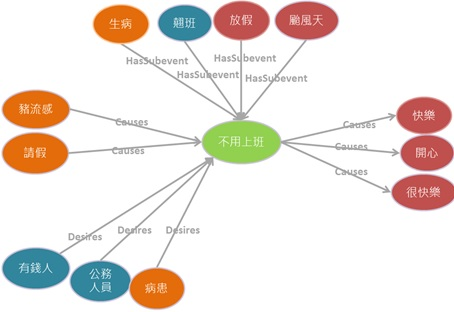
\includegraphics[width=2.5in]{fig/noWork2.jpg}
\caption{Neighbors of 'do not have to work' come from different scenarios.}
\label{fig:noWork2}
\end{figure}

The second problem is that each {\it concept} should be assigned different sentiments in different scenarios. For example, 'scream' is more possible to be negative when 'pervert' or 'cockroach' appears, but is more likely to be positive when 'idol' or 'win' appears. Previous approaches ~\cite{Xu:PACLIC10, Xu:COLING10, Rao:WWW14} use domain-specific corpus to modify sentiment value according to the corpus. However, hidden contextual information in Chinese ConceptNet is also abundant, like Figure~\ref{fig:noWork2}. If we could know which scenario an assertion belongs to, a {\it concept}'s sentiment in a scenario can be determined from its assertions which belongs to the scenario. 

To deal with the two problems, this paper develops a topic-aware propagation method for Chinese ConceptNet. We extract hidden contextual information by applying Latent Dirichlet Allocation~\cite{Blei:LDA03} to Chinese ConceptNet. Then we use the information to improve original sentiment propagation and predict topic-aware sentiment values for {\it concepts}. Then we present how to apply these topic-aware sentiment values of {\it concepts} to polarity classification for texts. Finally, experiments are conducted on dialogue dataset and microblog posts benchmark.


\section{Related Work}
\label{sec:relatedwork}
\subsection{Building Sentiment Dictionaries}
\subsubsection{Manually}
One way to build a sentiment dictionary is human annotation. The Affective Norms for English Words (ANEW) ~\cite{Bradley:ANEW99} is compiled manually and provides a set of normative ratings for 1034 English words. Bradley and Lang asked a group of Introductory Psychology class students to rate words in the ANEW through a normative rating procedure. They describe emotion using PAD emotional state model, and 

They use a picture-oriented instrument called the Self-Assessment Manikin (SAM) ~\cite{Lang:behavioral80} as the affective rating system to collect the pleasure, arousal, and dominance information for words. Although the sentiment values labelled by humans have high quality, the cost of collecting these labels is high. As the result, the coverage of words is limited.

\subsubsection{Sentiment Propagation}
Random walk is commonly used to spread sentiment values on a semantic graph~\cite{Wu:relSelect14, Hassan:ACL10, Xu:COLING10, Cambria:AAAI10}. Sentiment values are propagated through sentiment related edges, such as synonym and antonym relation. The equation of random walk with restart is as follows:
\begin{equation}
\label{eq:rndWalk}
\boldsymbol{s}_{t+1} = (1-\alpha)\boldsymbol{W}\boldsymbol{s}_t + \alpha\boldsymbol{s}_0
\end{equation}
where $\boldsymbol{s}_t$ is the values of each node when $t$-th iteration. $\boldsymbol{W}$ is a similarity matrix, which can be acquired from sources like Ontology, ConceptNet, corpus, etc. Similarity matrix of a standard random walk is an out-link normalized matrix. $\alpha$ is the restarting weight. Random walk is an iterative process, and after $n$ iteration, each node spreads its value to the neighbors that are $n$ links distant from it.

Besides terms, concepts like ``eat lunch", ``satisfy hunger" are associated with sentiments. Because the coverage of nodes in ConceptNet contains not only lexical terms but also such higher-order compound concepts, there are approaches proposed to predict sentiment values for nodes in ConceptNet~\cite{Liu:IUI03, Cambria:AAAI10, Wu:TAAI11, Tsai:IEEE13, Wu:relSelect14}. In ~\cite{Tsai:IEEE13, Wu:relSelect14}, random walk is applied to propagate sentiment values through relations of ConceptNet. They found that in ConceptNet, performing in-link normalized on similarity matrix is better than performing out-link normalized because out-link normalization will underestimate the influence of concepts with more neighbors. In in-link normalization, each concept's new sentiment value in the ($t+1$)-th iteration is the average of all its neighbors in the $t$-th iteration. However, in ConceptNet, a concept's neighbors may come from different situations, but this is not considered.

\subsubsection{Context-Aware Sentiment Dictionaries}
In most sentiment dictionaries, each term or phrase is associated with one sentiment value. However, the sentiment value should be different in different contexts or domains. For example, ``scream" is both possible to be positive and negative. ``huge" is positive in the sentence ``the room is huge", but is negative in the sentence ``the price is huge".

Common approaches aiming to build context-aware sentiment dictionaries rely on corpus and heuristic rules of sentences~\cite{Xu:PACLIC10, Xu:COLING10, Lu:WWW11}. They use the structures of sentences to construct relationship between words, such as ``and" being synonym and ``but" being antonym. There is another approach~\cite{Boia:AAAI14} using game to acquire contexts and sentiments of ambiguous phrases. 

Rao et al.~\cite{Rao:WWW14} use topic model to analyze co-occurrence information of the given news corpus and infer the topic distribution of each article. Combined with emotion labels, they can generate a sentiment dictionary which associates a sentiment value with each topic. 

Besides corpus, ConceptNet also has abundant contextual information. The semantic relations between concepts can also be used to propagate sentiments, which are not limited to synonym or antonym. For example, ``get F score Causes sad" tells us the sentiment of concept ``get F score" is related to the concept ``sad" because of the relation ``Causes". As the result, our approach relies on contextual information and structure of ConceptNet.



\section{Topic-Aware Sentiment Value Prediction for Chinese ConceptNet}
\label{sec:method1}
In topic models such as LDA, each abstract ``topic" is characterized by a distribution over words. Such topics are one kind of representation of contexts or scenarios. In this section, we aim to define the topics in Chinese ConceptNet and predict a sentiment value $\in [-1,1]$ on each topic for each concept. Figure~\ref{fig:system1} shows the architecture of our system.

\begin{figure}[!t]
\centering
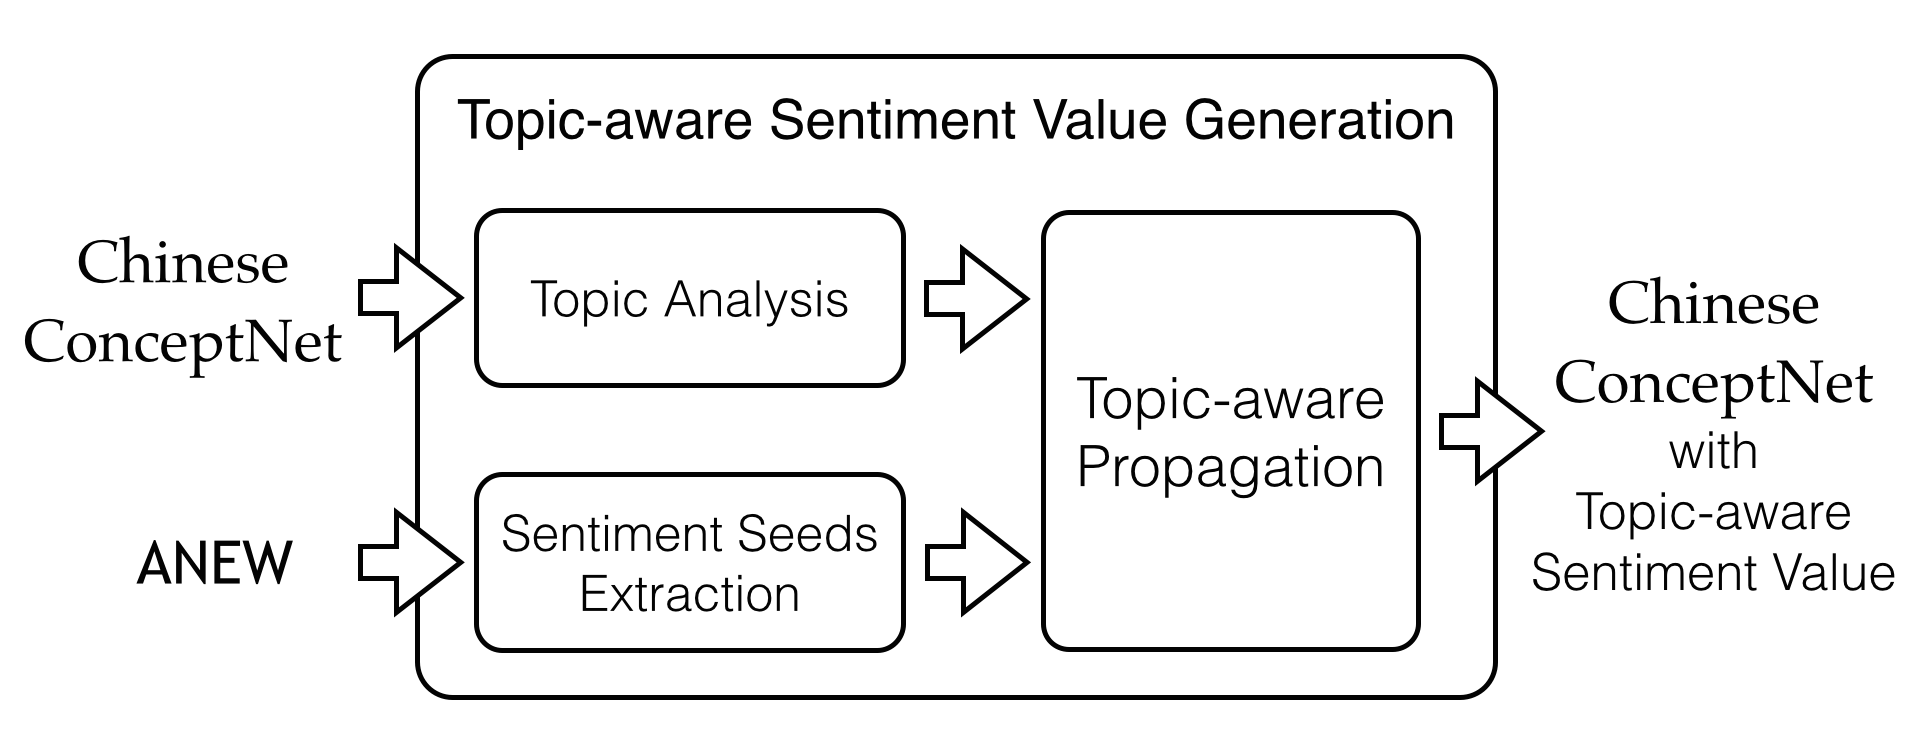
\includegraphics[width=0.5\textwidth]{fig/system1.png}
\caption{System Architecture.}
\label{fig:system1}
\end{figure}

\subsection{Topic Analysis on ConceptNet}
We choose LDA to estimate topics for two reasons: The first one is that LDA allows each document to exhibit multiple topics to different degrees. The second one is that there are corpus parameters after LDA estimation, and we can use these corpus parameters to infer a new document by running the E-step in LDA. 

Similar to the assumption of generating a corpus in LDA, we assume that there is a topic distribution for each concept and its assertions are sampled from this distribution. We aim to find which topic each assertion comes from for each concept. Therefore, we try to apply LDA to find such latent information. 

First, each concept forms a document using its neighbors such that these neighbors have one co-occurrence observation when LDA estimates. See Figure~\ref{fig:noWorkDoc} for illustration, the concept 'do not have to work' generates a document using neighbors as words, with a value indicating how many times the neighbor occurs in assertions.

\begin{figure}[!t]
\centering
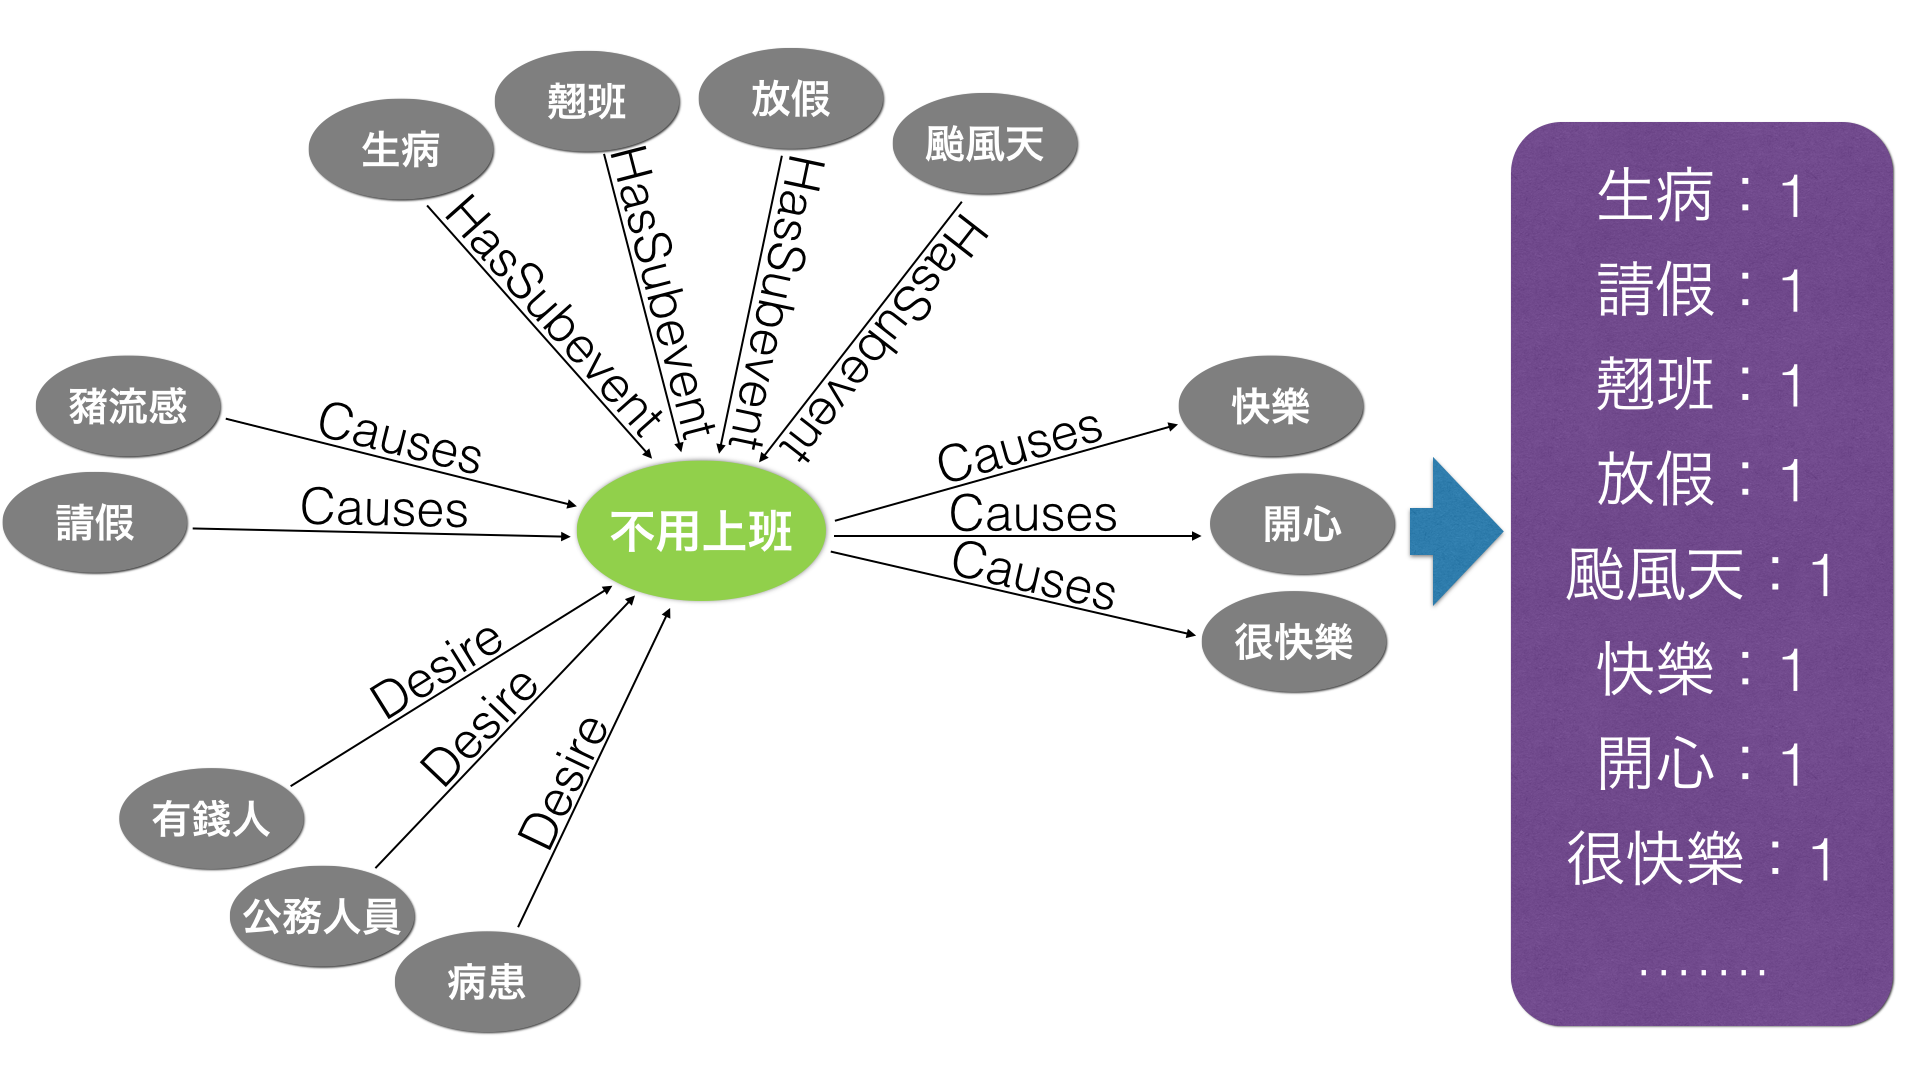
\includegraphics[width=0.5\textwidth]{fig/noWorkDoc.png}
\caption{The document generated by 'do not have to work'.}
\label{fig:noWorkDoc}
\end{figure}

Then we apply LDA to find $\boldsymbol{\theta}_m$ for each document d$_m$ and $z_{m,n}$ for each word $w_{m,n}$ in d$_m$ based on this collection of $M$ documents. Words in each document stand for neighbors of concept, so each resulted $z_{m,n}$ indicates which topicID the neighbor $w_{m,n}$ comes from for concept $c_m$.

As the result, we can design a topic assignment matrix, $\boldsymbol{T}$ where each entry $t_{i,j}$ is $z_{i,j}$ if $j$ is one of $i$'s neighbors, otherwise $unknown$. That is, we can check $t_{i,j}$ for which topicID $i$'s neighbor $j$ belongs to. 

Here we present the result of applying LDA with 10 topics to Chinese ConceptNet. Figure~\ref{fig:wordTop20} shows the per-topic word distribution, $\boldsymbol{\beta}_k$. Each column shows the top 20 words of a topic.

\begin{figure}[!t]
\centering
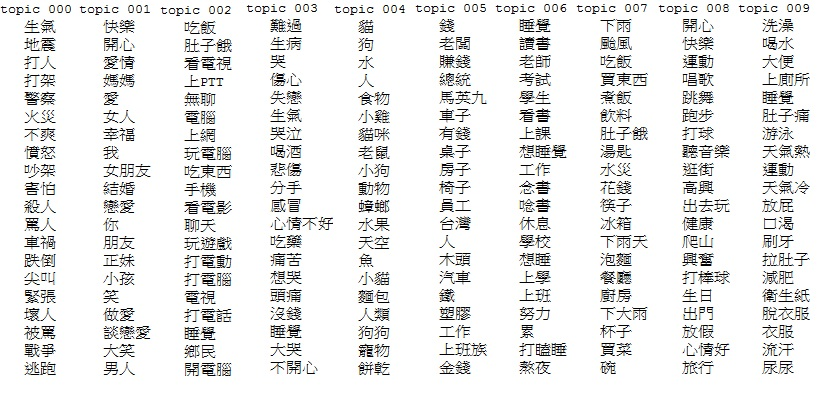
\includegraphics[width=0.5\textwidth]{fig/wordTop20.jpg}
\caption{The top 20 words of each topic.}
\label{fig:wordTop20}
\end{figure}

\subsection{Sentiment Seeds Extraction}
Sentiment seeds here are concepts whose sentiments are known. Common ways to collect sentiment seeds are compiling manually or using other existing sentiment dictionaries. Although concepts we consider here are in Chinese, we use words in Affective Norms for English Words (ANEW)~\cite{Bradley:ANEW99} as our seeds. One reason is its good quality: it was compiled manually by a group of Introductory Psychology class students and provides ratings for 1034 English words through a normative rating procedure. Another reason is that sentiments in ANEW is value-level. Value-level sentiments provide additional intensity information.

We want to assign each concept a sentiment value $\in [-1,1]$ measuring how pleasant or unpleasant people feel about it, so we use the value in ``Pleasure" dimension. Values in ANEW are $\in [1,9]$, so we perform linear normalization on them to value $\in [-1,1]$.

We apply Google Translate to translate all 1034 words in ANEW into Chinese. There may be multiple translations of a English word, we take all of them into account and verify manually. We verify whether the polarities of a English word and its translations are similar. To match more concepts in Chinese ConceptNet, we expand these translations by the approach in our previous research~\cite{Wu:TAAI11}. After expansion, we have 27842 Chinese phrases with sentiment values. In our experiment, there are totally 3047 of them match concepts in Chinese ConceptNet, and then these concepts are used as sentiment seeds.

As the result, given totally $M$ concepts in ConceptNet, we generate a $M \times 1$ vector $\boldsymbol{s}_0$ to denote sentiment values of seed concepts. For each phrase in our expanded translations, if it appears in ConceptNet with concept ID $c$, the ($c$,1) entry of $\boldsymbol{s}_0$ is its linear normalized sentiment value in ANEW. Other entries are $unknown$.

\subsection{Topic-Aware Sentiment Propagation}
After topic analysis, we know which topic each neighbor of each concept comes from by topic assignment matrix $\boldsymbol{T}$. When we predict $c_m$'s sentiment value on the latent topic $z$, we consider neighbors which come from topic $z$ and use their sentiment values on topic $z$. 

However, not all assertions are good for propagation. Next, We select sentiment related relation types and their directions by validation. More specifically, 10\% of positive/neutral/negative sentiment seeds are sampled as validation, and use the remaining 90\% to propagate. The result is shown in Table~\ref{table:relRule}.

\begin{table}[]
\centering
\caption{Propagation rules on 13 relation types}
\label{table:relRule}
\begin{tabular}{|l|l|}
\hline
Relation Type    & Propagation rule  \\ \hline
HasFirstSubevent & Not used  		 \\ \hline
MadeOf 			 & Not used  		 \\ \hline
IsA 			 & Not used  		 \\ \hline
AtLocation 		 & Not used  		 \\ \hline
UsedFor 		 & Not used  		 \\ \hline
CapableOf 		 & Not used  		 \\ \hline
MotivatedByGoal  & Latter to Former  \\ \hline
Desires 		 & Not used          \\ \hline
SymbolOf 		 & Former to Latter  \\ \hline
CausesDesire 	 & Not used  		 \\ \hline
Causes 			 & Both Direction    \\ \hline
HasSubevent      & Former to Latter  \\ \hline
PartOf           & Not used  		 \\ \hline
\end{tabular}
\end{table}

Starting from seed concepts, we can use equation~\ref{eq:rndWalk} to iteratively propagate sentiment values on different topics. We design $\boldsymbol{W}$, the $M \times M$ propagation matrix by Algorithm~\ref{alg:wmatrix}. Each element $w_{i,j}$ denotes the weight of sentiment value propagation from concept $j$ to concept $i$.

\begin{algorithm}[htb]
  \caption{determine $\boldsymbol{W}$ for a given topic $z$}
  \label{alg:wmatrix}
  \begin{algorithmic}[1]
  	\Require
  		$z$: current topicID; 
  		$\boldsymbol{T}$: topic assignment matrix;
  		$\text{A} = \{(c1,c2,rel)\}$: all ConceptNet assertions;
    \Ensure
     	$M \times M$ propagation matrix $\boldsymbol{W}$;
	\State initialize $M \times M$ matrix $\boldsymbol{W}$ with each entry $w_{i,j} = 0$    
    \For{each assertion $(c_i,c_j,rel)$ in A}
    \label{code:ruleStart}
    	\State rule = searchPropagationRule($(c_i,c_j,rel)$);
		\If{rule = ``Former to Latter"}
			\State $w_{j,i} \pluseq 1$;
		\ElsIf{rule = ``Latter to Former"}
			\State $w_{i,j} \pluseq 1$;
		\ElsIf{rule = ``Both Direction"}
			\State $w_{j,i} \pluseq 1$, $w_{i,j} \pluseq 1$;
		\EndIf
	\EndFor
	\label{code:ruleEnd}
    
    \For{each $t_{i,j}$ in $\boldsymbol{T}$}
    \label{code:separateContextStart}
		\If{$t_{i,j} \neq z$}
			$w_{i,j} = 0$;
			\Comment{For concept $i$, consider only neighbors in topic $z$}
		\EndIf
    \EndFor
    \label{code:separateContextEnd}
    \State \Return $\boldsymbol{W}$;
  \end{algorithmic}
\end{algorithm}

We can design the propagation matrix for each topic and use it to propagate sentiment values separately. No matter which topic, propagation starts from $\boldsymbol{s}_0$ because the seeds are less ambiguous on different topics. In each iteration $i$, we perform in-link normalization to the propagation matrix. After propagating $iteration$ times, we have the final $\boldsymbol{s}_{iteration}$, which stands for the final sentiment values on topic $z$ for all concepts in ConceptNet. We set sentiment value to $0$ for concepts which are still labelled $unknown$ in $\boldsymbol{s}_{iteration}$. Then, this process repeats for other topics. Finally, each concept has a sentiment value $\in [-1,1]$ on each topic.



\section{Topic Inference and Sentiment Value Selection}
\label{sec:method2}
When predicting polarities for texts, concepts in the texts provide important information. For example, if 'F score', 'sad' and 'die' co-occur in a text, the text is more likely to be negative. We claim that when we want to know a concept's sentiment value, it's better to return a value based on the current topic, rather than a fixed value. For example, in the sentence 'The case is too sudden', 'sudden' reflects sentiment, but it is both possible to be positive and negative depending on the description about 'the case'. The description may consist of concepts such as 'surprise', 'nervous' and 'help'. Hence, we use co-occurring concepts to help us identify topics and sentiment values for a concept in texts.

That is, given a query concepts $c_q$ and a set of co-occurring concepts COO $= \{(c_i, count_i) \mid c_i$ occurs $count_i$ times$\}$, the output is $(topic, val)$ where $topic$ is the topicID $c_q$ most likely belong to, and $val$ is the sentiment value $\in [-1, 1]$ of $c_q$ when $topic$.

First, we combine $c_q$ and COO to form a document d$_q$, which is a set of tuples $(c_i, count_i)$ indicating $c_i$ occurs $count_i$ times in $c_q$ and COO. Next, we use the corpus LDA parameters $\boldsymbol{\alpha}$ and $\boldsymbol{\beta}_k$ trained using ConceptNet to infer d$_q$. By running the E-step, LDA estimates topic distribution of d$_q$ and the topic assignments for concepts in d$_q$. As the result, we know which topics $c_q$ and COO come from, and use the topic of $c_q$ to access the topic-aware sentiment results in section~\ref{sec:method1}. Finally, the most possible topic and sentiment value of $c_q$ is returned.






\section{Experiments}
\label{sec:experiment}
\subsection{Experimental Setup}
In our experiment, we use the Chinese part of ConceptNet which we collect by ChickenPTT~\cite{Kuo:HCOMP09} until May, 19, 2015. There are totally 713139 assertions and 223871 concepts. 

ANEW is used as our seeds. There are 1034 English words in ANEW. After our translation and expansion, these English words generate 27842 Chinese phrases. There are 3047 of them existing in ConceptNet. Among these 3047 concepts, there are 1654 positive, 1042 negative, 351 neutral according to sentiment values in ANEW. (After linear normalization, we define neutral using $\pm0.125$ as threshold.)

\subsection{Experiment 1: Propagation on the Same Topic}
This experiment aims to evaluate whether propagating on each topic separately is better than the original method which decides sentiment values from all neighbors together disregarding topics.

\subsubsection{Test Data}
From 3047 seed concepts, we sample 10\% of them to evaluate our propagation result and use the remaining 90\% as propagation seeds. To make the distributions of 10\% test data and the 90\% training data similar, we sample test data according to the proportions of positive, neutral and negative concepts. Therefore, in the test set there are totally 304 concepts where 165 of them are positive, 104 of them are negative and 35 of them are neutral.

\subsubsection{Evaluation Metrics}
We use point-wise accuracy and pair-wise accuracy to evaluate. Point-wise accuracy measures the proportion of concepts whose predicted polarities are same as their ground-truth to all test concepts. Pair-wise accuracy measures the proportion of pairs of concepts which have the same relative relation as ground-truth to all pairs.

\subsubsection{Post-Processing}
In our topic-aware results, each concept has different sentiment values on different topics. That is, each concept is associated with multiple sentiment values. To compare with original propagation, we aggregate values on different topics into one value. We compute a weighted arithmetic mean over sentiments on different topics. The weight of sentiment on topic $z$ is the proportion of valid neighbors belonging to $z$ among all valid neighbors.

\subsubsection{Results and Discussion}
The results of topic-insensitive and topic-aware propagation are discussed here. The former is the baseline, and we compare it with our topic-aware propagations with different topic numbers.

The results of point-wise and pair-wise accuracy are shown in Fig~\ref{fig:exp1_iter_pointAcc} and Fig~\ref{fig:exp1_iter_pairAcc} respectively. We can see that the performance of baseline become worse when propagating sentiments to more concepts. In contrast, topic-aware propagations with topic number $>2$ have higher and more stable point-wise accuracy and pairwise accuracy as iteration goes.

Here we investigate topic number $<=10$. Larger topic number causes topic layers of Chinese ConceptNet sparse and makes sentiment propagation fail. We found generalize contextual information into $<=10$ topics performs better.

\begin{figure}[!t]
\centering
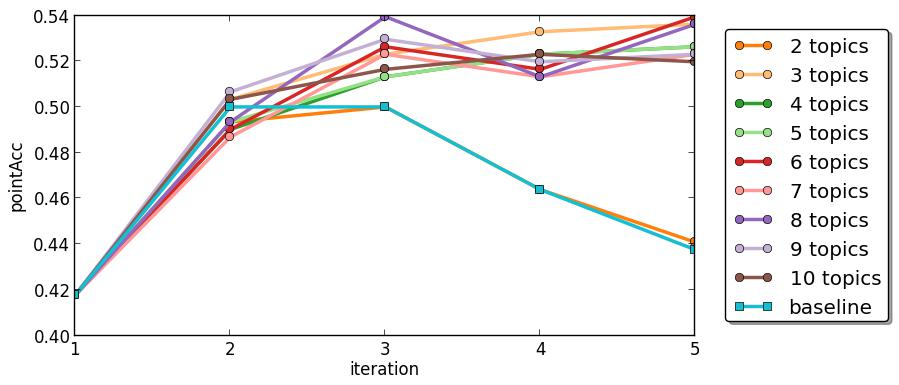
\includegraphics[width=3in]{fig/exp1_iterations/pointAcc.jpg}
\caption{Point-wise accuracy of all test concepts for the first 5 iterations.}
\label{fig:exp1_iter_pointAcc}
\end{figure}

\begin{figure}[!t]
\centering
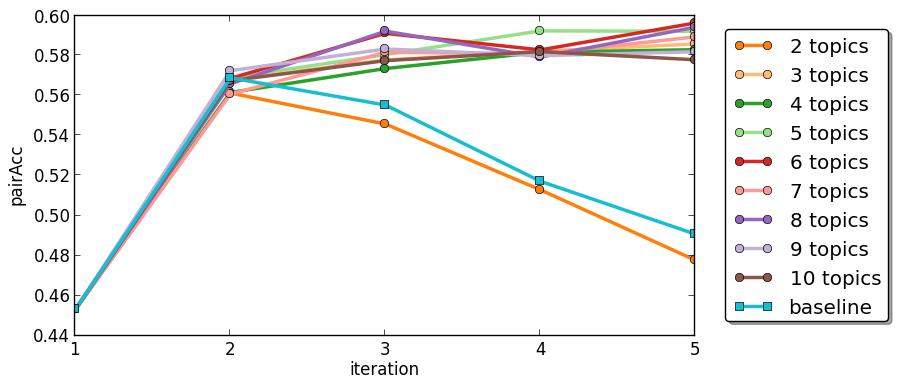
\includegraphics[width=3in]{fig/exp1_iterations/pairAcc.jpg}
\caption{Pairwise accuracy of all test concepts for the first 5 iterations.}
\label{fig:exp1_iter_pairAcc}
\end{figure}

\begin{figure}[!t]
\centering
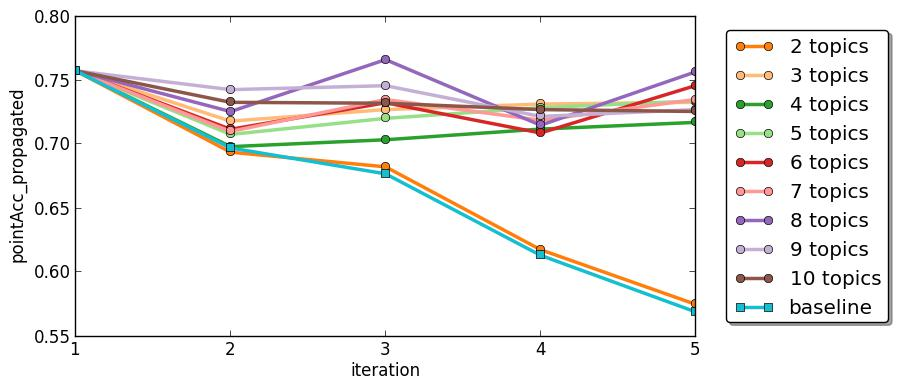
\includegraphics[width=3in]{fig/exp1_iterations/pointAcc_propagated.jpg}
\caption{Point-wise accuracy of test concepts propagated for the first 5 iterations.}
\label{fig:exp1_iter_pointAcc_known}
\end{figure}

\begin{figure}[!t]
\centering
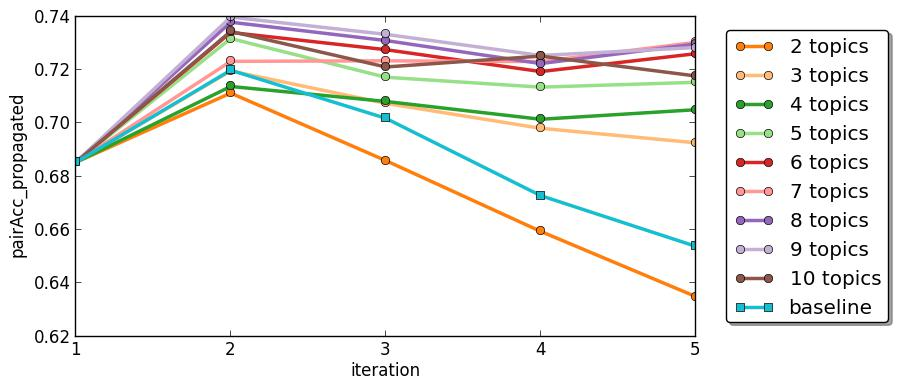
\includegraphics[width=3in]{fig/exp1_iterations/pairAcc_propagated.jpg}
\caption{Pairwise accuracy of all test concepts propagated for the first 5 iterations.}
\label{fig:exp1_iter_pairAcc_known}
\end{figure}

Some of test concepts didn't get sentiment values when propagation and are considered as neutral in our system. We exclude these concepts and investigate the performance of the remaining concepts for each iteration in Fig~\ref{fig:exp1_iter_pointAcc_known} and Fig~\ref{fig:exp1_iter_pairAcc_known}. The point-wise accuracy and pairwise accuracy reach 0.7. Except the topic number $=2$ one, topic-aware ones have higher accuracies.


%===========================
\subsection{Experiment 2: Polarity Classification for Posts of Microblog}
This experiment aims to investigate the effect of using topic-aware sentiments of concepts to predict polarities of texts. 

\subsubsection{Test Data}
The benchmark dataset is from the Chinese Microblog Sentiment Analysis Evaluation (CMSAE) task in the conference on Natural Language Processing \& Chinese Computing (NLP \& CC) 2013 \footnote{\url{http://tcci.ccf.org.cn/conference/2013/pages/page04_dg.html}}.

The original task in NLP \& CC is to recognize the emotion types of Chinese microblog texts collected from Sina Weibo. The seven emotion types are: {\it anger}, {\it disgust}, {\it fear}, {\it happiness}, {\it like}, {\it sadness}, and {\it surprise}. If the text has no emotion, it is labelled as {\it none}. The test dataset contains 10000 microblog texts and 32185 sentences. Each text is labelled a primary emotion type and a possible secondary emotion type. 

Because our system is designed for recognizing the polarity, we reduce the emotion types into polarities. The emotion types {\it anger}, {\it disgust}, {\it fear} and {\it sadness} are mapped to {\it negative}. The emotion types {\it happiness} and {\it like} are mapped to {\it positive}. We map {\it surprise} and {\it none} to {\it neutral}. For each text, we use the primary emotion as its label. We use the secondary emotion as its label only when the primary emotion is {\it neutral}. For example, if a text is labelled {\it surprise} (primary) and {\it disgust} (secondary), its polarity is {\it negative}. The distribution of microblog texts is shown in TABLE~\ref{table:microblogDist}.

\begin{table}[!t]
\centering
\caption{Distribution of Chinese microblog texts in the test set}
\label{table:microblogDist}
\begin{tabular}{|l|l|l|l|}
\hline
positive & neutral & negative & total \\ \hline
2235 & 1913 & 5852 & 10000  \\ \hline
\end{tabular}
\end{table} 

\subsubsection{Evaluation Metrics}
Following the task in NLP \& CC, we use the macro average and micro average on precision, recall and F-measure to evaluate.

\begin{equation}
\label{eq:macroPrec}
\text{Macro\_Precision} = \frac{1}{3} \sum_{i} \frac{\#system\_correct(polarity=i)}{\#system\_proposed(polarity=i)}
\end{equation}

\begin{equation}
\label{eq:macroRecall}
\text{Macro\_Recall} = \frac{1}{3} \sum_{i} \frac{\#system\_correct(polarity=i)}{\#gold\_standard(polarity=i)}
\end{equation}

\begin{equation}
\label{eq:macroF}
\text{Macro\_F-measure} = \frac{2 \times Macro\_Precision \times Macro\_Recall}{Macro\_Precision+Macro\_Recall}
\end{equation}

\begin{equation}
\label{eq:microPrec}
\text{Micro\_Precision} = \frac{\sum_{i}\#system\_correct(polarity=i)}{\sum_{i}\#system\_proposed(polarity=i)}
\end{equation}

\begin{equation}
\label{eq:microRecall}
\text{Micro\_Recall} = \frac{\sum_{i}\#system\_correct(polarity=i)}{\sum_{i}\#gold\_standard(polarity=i)}
\end{equation}

\begin{equation}
\label{eq:microF}
\text{Micro\_F-measure} = \frac{2 \times Micro\_Precision \times Micro\_Recall}{Micro\_Precision+Micro\_Recall}
\end{equation}

\subsubsection{Lexicon Based Polarity Prediction}
We predict the polarity for each post by a basic lexicon based approach. We use Chinese text segmentation tool jieba~\footnote{https://pypi.python.org/pypi/jieba/0.37} to sentences in the post and find words or phrases appearing in ConceptNet. 

Here we compare the performance of concepts' sentiments generated by methods in TABLE~\ref{table:comparePredict}. For methods which associates each concept with one sentiment value, we compare both performance of iteration 2 and 5. The iteration 2 is more conservative while the iteration 5 is more aggressive. In M2, we use the concepts in all sentences in the post as co-occurring concepts, and the system will return the topic and sentiment value for each concept. Because we observe that topic-aware propagation is more effective as iteration goes, M2 use the result when iteration $=5$. 

\begin{table}[!t]
\centering
\caption{Methods to predict polarities of dialogues}
\label{table:comparePredict}
\begin{tabular}{|l|l|}
\hline
Method    & Explanation  \\ \hline
Baseline-iteration2 or 5 & \makecell[l]{In-link propagation with relation rules} \\ \hline
M1-iteration2 or 5 & \makecell[l]{Baseline + Topic based propagation \\ $\rightarrow$ each concept associated with \\ one sentiment value} \\ \hline
M2 & \makecell[l]{Baseline + Topic based propagation \\ $\rightarrow$ each concept has different \\ sentiment values on different topics} \\ \hline
\end{tabular}
\end{table}

After knowing the sentiment values of concepts in posts, we define commonly used negation words. Then we use negation words to negate the sentiment values of those concepts behind it. Finally, all sentiment values are summed up, and we use its sign as the polarity of this post. ($\pm 0.125$ as the threshold of neutral) 

\subsubsection{Results and Discussion}
The performance of M2 using different topic number is shown in TABLE~\ref{table:microblogM2}. M2 using more topics performs better. TABLE~\ref{table:microblogM1_2} and TABLE~\ref{table:microblogM1_5} are results of using M1-iteration2 and M1-iteration5 respectively. TABLE~\ref{table:microblogbase} shows the results of baseline. We can see that the results of M2 are generally better than them. This shows the effectiveness of our topic-aware approach. 

\begin{table}[!t]
\centering
\caption{Results of using M2}
\label{table:microblogM2}
\begin{tabular}{|l|l|l|l|l|l|l|}
\hline
\multirow{2}{*}{Method} & \multicolumn{3}{|l|}{macro-average} & \multicolumn{3}{|l|}{micro-average} \\ \cline{2-7}
& prec & recall & F score & prec & recall & F score \\ \hline
2 topics & 0.342 & 0.371 & 0.356 & 0.469 & 0.469 & 0.469 \\ \hline
3 topics & 0.356 & 0.345 & 0.350 & 0.462 & 0.462 & 0.462 \\ \hline
4 topics & 0.363 & 0.365 & 0.364 & 0.421 & 0.421 & 0.421 \\ \hline
5 topics & 0.399 & 0.392 & 0.396 & 0.487 & 0.487 & 0.487 \\ \hline
6 topics & 0.390 & 0.390 & 0.390 & 0.472 & 0.472 & 0.472 \\ \hline
7 topics & 0.420 & 0.404 & 0.412 & 0.516 & 0.516 & 0.516 \\ \hline
8 topics & 0.420 & 0.404 & 0.411 & 0.527 & 0.527 & 0.527 \\ \hline
9 topics & 0.427 & 0.402 & 0.414 & 0.534 & 0.534 & 0.534 \\ \hline
10 topics & 0.433 & 0.406 & 0.419 & 0.524 & 0.524 & 0.524 \\ \hline
\end{tabular}
\end{table}

\begin{table}[!t]
\centering
\caption{Results of using M1-iteration2}
\label{table:microblogM1_2}
\begin{tabular}{|l|l|l|l|l|l|l|}
\hline
\multirow{2}{*}{Method} & \multicolumn{3}{|l|}{macro-average} & \multicolumn{3}{|l|}{micro-average} \\ \cline{2-7}
& prec & recall & F score & prec & recall & F score \\ \hline
2 topics & 0.377 & 0.367 & 0.372 & 0.251 & 0.251 & 0.251 \\ \hline
3 topics & 0.367 & 0.371 & 0.369 & 0.254 & 0.254 & 0.254 \\ \hline
4 topics & 0.388 & 0.377 & 0.382 & 0.257 & 0.257 & 0.257 \\ \hline
5 topics & 0.365 & 0.378 & 0.372 & 0.258 & 0.258 & 0.258 \\ \hline
6 topics & 0.378 & 0.375 & 0.377 & 0.255 & 0.255 & 0.255 \\ \hline
7 topics & 0.364 & 0.378 & 0.370 & 0.257 & 0.257 & 0.257 \\ \hline
8 topics & 0.366 & 0.381 & 0.373 & 0.261 & 0.261 & 0.261 \\ \hline
9 topics & 0.376 & 0.384 & 0.380 & 0.263 & 0.263 & 0.263 \\ \hline
10 topics & 0.380 & 0.380 & 0.380 & 0.260 & 0.260 & 0.260 \\ \hline
\end{tabular}
\end{table} 

\begin{table}[!t]
\centering
\caption{Results of using M1-iteration5}
\label{table:microblogM1_5}
\begin{tabular}{|l|l|l|l|l|l|l|}
\hline
\multirow{2}{*}{Method} & \multicolumn{3}{|l|}{macro-average} & \multicolumn{3}{|l|}{micro-average} \\ \cline{2-7}
& prec & recall & F score & prec & recall & F score \\ \hline
2 topics & 0.365 & 0.352 & 0.358 & 0.242 & 0.242 & 0.242 \\ \hline
3 topics & 0.374 & 0.369 & 0.372 & 0.256 & 0.256 & 0.256 \\ \hline
4 topics & 0.361 & 0.373 & 0.367 & 0.253 & 0.253 & 0.253 \\ \hline
5 topics & 0.372 & 0.382 & 0.377 & 0.260 & 0.260 & 0.260 \\ \hline
6 topics & 0.366 & 0.377 & 0.371 & 0.257 & 0.257 & 0.257 \\ \hline
7 topics & 0.369 & 0.381 & 0.375 & 0.261 & 0.261 & 0.261 \\ \hline
8 topics & 0.388 & 0.386 & 0.387 & 0.265 & 0.265 & 0.265 \\ \hline
9 topics & 0.383 & 0.389 & 0.386 & 0.266 & 0.266 & 0.266 \\ \hline
10 topics & 0.368 & 0.377 & 0.372 & 0.258 & 0.258 & 0.258 \\ \hline
\end{tabular}
\end{table}

\begin{table}[!t]
\centering
\caption{Results of using Baseline-iteration2 and 5}
\label{table:microblogbase}
\begin{tabular}{|l|l|l|l|l|l|l|}
\hline
\multirow{2}{*}{Method} & \multicolumn{3}{|l|}{macro-average} & \multicolumn{3}{|l|}{micro-average} \\ \cline{2-7}
& prec & recall & F score & prec & recall & F score \\ \hline
iteration2 & 0.386 & 0.358 & 0.372 & 0.244 & 0.244 & 0.244 \\ \hline
iteration5 & 0.355 & 0.349 & 0.352 & 0.238 & 0.238 & 0.238 \\ \hline
\end{tabular}
\end{table}



% An example of a floating figure using the graphicx package.
% Note that \label must occur AFTER (or within) \caption.
% For figures, \caption should occur after the \includegraphics.
% Note that IEEEtran v1.7 and later has special internal code that
% is designed to preserve the operation of \label within \caption
% even when the captionsoff option is in effect. However, because
% of issues like this, it may be the safest practice to put all your
% \label just after \caption rather than within \caption{}.
%
% Reminder: the "draftcls" or "draftclsnofoot", not "draft", class
% option should be used if it is desired that the figures are to be
% displayed while in draft mode.
%
%\begin{figure}[!t]
%\centering
%\includegraphics[width=2.5in]{myfigure}
% where an .eps filename suffix will be assumed under latex, 
% and a .pdf suffix will be assumed for pdflatex; or what has been declared
% via \DeclareGraphicsExtensions.
%\caption{Simulation results for the network.}
%\label{fig_sim}
%\end{figure}

% Note that IEEE typically puts floats only at the top, even when this
% results in a large percentage of a column being occupied by floats.


% An example of a double column floating figure using two subfigures.
% (The subfig.sty package must be loaded for this to work.)
% The subfigure \label commands are set within each subfloat command,
% and the \label for the overall figure must come after \caption.
% \hfil is used as a separator to get equal spacing.
% Watch out that the combined width of all the subfigures on a 
% line do not exceed the text width or a line break will occur.
%
%\begin{figure*}[!t]
%\centering
%\subfloat[Case I]{\includegraphics[width=2.5in]{box}%
%\label{fig_first_case}}
%\hfil
%\subfloat[Case II]{\includegraphics[width=2.5in]{box}%
%\label{fig_second_case}}
%\caption{Simulation results for the network.}
%\label{fig_sim}
%\end{figure*}
%
% Note that often IEEE papers with subfigures do not employ subfigure
% captions (using the optional argument to \subfloat[]), but instead will
% reference/describe all of them (a), (b), etc., within the main caption.
% Be aware that for subfig.sty to generate the (a), (b), etc., subfigure
% labels, the optional argument to \subfloat must be present. If a
% subcaption is not desired, just leave its contents blank,
% e.g., \subfloat[].


% An example of a floating table. Note that, for IEEE style tables, the
% \caption command should come BEFORE the table and, given that table
% captions serve much like titles, are usually capitalized except for words
% such as a, an, and, as, at, but, by, for, in, nor, of, on, or, the, to
% and up, which are usually not capitalized unless they are the first or
% last word of the caption. Table text will default to \footnotesize as
% IEEE normally uses this smaller font for tables.
% The \label must come after \caption as always.
%
%\begin{table}[!t]
%% increase table row spacing, adjust to taste
%\renewcommand{\arraystretch}{1.3}
% if using array.sty, it might be a good idea to tweak the value of
% \extrarowheight as needed to properly center the text within the cells
%\caption{An Example of a Table}
%\label{table_example}
%\centering
%% Some packages, such as MDW tools, offer better commands for making tables
%% than the plain LaTeX2e tabular which is used here.
%\begin{tabular}{|c||c|}
%\hline
%One & Two\\
%\hline
%Three & Four\\
%\hline
%\end{tabular}
%\end{table}


% Note that the IEEE does not put floats in the very first column
% - or typically anywhere on the first page for that matter. Also,
% in-text middle ("here") positioning is typically not used, but it
% is allowed and encouraged for Computer Society conferences (but
% not Computer Society journals). Most IEEE journals/conferences use
% top floats exclusively. 
% Note that, LaTeX2e, unlike IEEE journals/conferences, places
% footnotes above bottom floats. This can be corrected via the
% \fnbelowfloat command of the stfloats package.




\section{Conclusion}
\label{sec:conclusion}
In this paper, a new method, topic-aware propagation, is proposed to estimate topic-aware sentiment values for nodes in Chinese ConceptNet. One contribution is that we propose separating neighbors by topics before propagation. The result shows that it performs better than running propagation directly. Another contribution is that we deal with the problem that the sentiment of concepts should depend on texts. Our topic-aware propagation can assign each concept different sentiment values on different topics. When predicting polarities for texts, our system will output the most possible topics and sentiment values for concepts in texts. 

In the experiment of predicting polarities for microblog posts, we simply apply negation rules and sum up sentiment values of concepts. However, a more elegant approach can be designed to utilize the topics and sentiments of concepts outputted by our system.




% conference papers do not normally have an appendix



% use section* for acknowledgment
%\ifCLASSOPTIONcompsoc
  % The Computer Society usually uses the plural form
%  \section*{Acknowledgments}
%\else
  % regular IEEE prefers the singular form
%  \section*{Acknowledgment}
%\fi




% trigger a \newpage just before the given reference
% number - used to balance the columns on the last page
% adjust value as needed - may need to be readjusted if
% the document is modified later
%\IEEEtriggeratref{8}
% The "triggered" command can be changed if desired:
%\IEEEtriggercmd{\enlargethispage{-5in}}

% references section

% can use a bibliography generated by BibTeX as a .bbl file
% BibTeX documentation can be easily obtained at:
% http://www.ctan.org/tex-archive/biblio/bibtex/contrib/doc/
% The IEEEtran BibTeX style support page is at:
% http://www.michaelshell.org/tex/ieeetran/bibtex/
\bibliographystyle{IEEEtran}
% argument is your BibTeX string definitions and bibliography database(s)
%\bibliography{IEEEabrv,../bib/paper}
%
% <OR> manually copy in the resultant .bbl file
% set second argument of \begin to the number of references
% (used to reserve space for the reference number labels box)
\bibliography{taaibib}




% that's all folks
\end{document}


